\section{Method}
The general idea is to generate the medial axis transform and round the distance measures,
such that an exact integer beads will fit the polygon there
so that there is never a gap region left over in the middle of the polygon.

We round to integer multiples of half the nozzle width so as to allow single-bead segments, rather than only having polygonal insets.

\begin{figure}
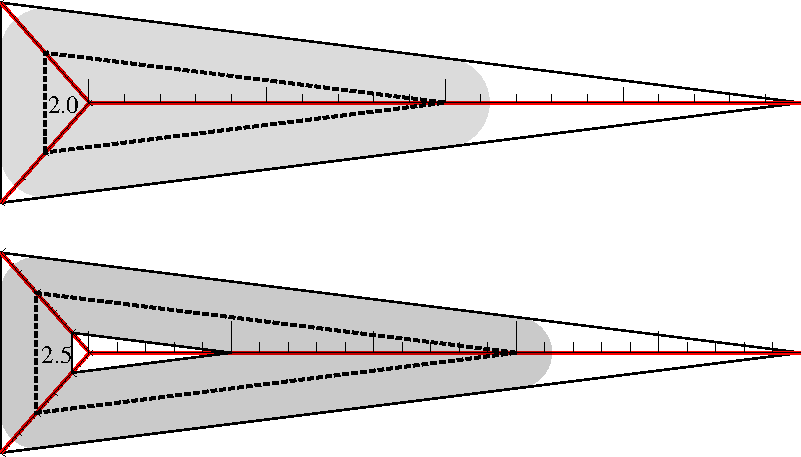
\includegraphics[width=\columnwidth]{sources/method/rounded_vs_unrounded.pdf}
\caption{Toolpaths employing dist rounding vs without.}
\label{rounded_vs_unrounded}
\end{figure}


\begin{figure}
\begin{subfigure}{0.45\columnwidth}
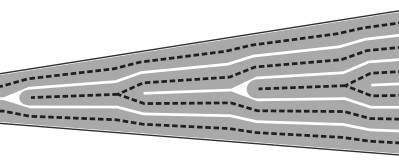
\includegraphics[width=\columnwidth]{sources/method/single_bead_strategy.jpg}
\caption{Overview}
\label{single_bead_strategy_overview}
\end{subfigure}
\begin{subfigure}{0.45\columnwidth}
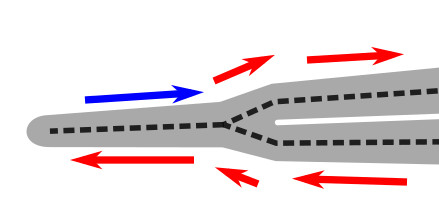
\includegraphics[width=\columnwidth]{sources/method/single_bead_strategy_order.jpg}
\caption{Travel order}s
\end{subfigure}
\caption{We can do single-bead segments. Blue is travel move.}
\label{single_bead_strategy}
\end{figure}

\old{
\subsection{Method Overview}
\begin{enumerate}
\item compute medial axis transform (MAT)
\item find places `of high curvature' in the medial axis and mark those regions
\item transform the $R$ distance measures in the marked regions to enable fitting an integer multiple beads.
		This transformation uses transition regions to smoothly transition from $n$ into $n+1$ insets.
\item introduce extra `joints' on the medial axis in order to discretize the transformed distance measure
\item connect these new joints to the outline with new `bones' (In the standard MAT manner)
\item (optional) transform $R$ fields along all bones, while keeping the endpoint bead measures fixed. (Deviate from evenly distributed linear space in order to have outer outlines closer to the nominal bead width and only change the innermost couple of toolpaths.)
\item define locations everywhere on the bones of the medial axis at integer MAT distances
\item connect all locations with odd distance measure to form the inset toolpaths
\item connect all even locations to form the extent of the toolpaths, which defines the variable width of the segments.
\end{enumerate}
}

\hl{Idea: generate only outer 3 walls, except in marked regions where the distance $R < 5 \win$, so as to prevent jagged infill lines.}
\Cref{wedge_and_infill}

\hl{Filter beading number in order to prevent regions with a lot of back and forth transitions.}

\subsection{Terminology}
For an explanation of the terms used, see \cref{legend}.

\begin{figure}
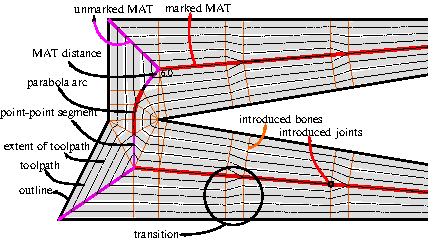
\includegraphics[width=\columnwidth]{sources/method/legend_double_wedge_example.pdf}
\caption{Explanation of terms.}
\label{legend}
\end{figure}



\hl{We need consistent terminology and symbols which adhere to standards in literature.}
The following synonym groups are used here which are not yet checked with existing literature':
\begin{itemize}
\item bones, medial axis segments, arms, fingers, ribs
\item joints, ticks, medial axis vertices, locations
\item MAT distance measure
\end{itemize}


Based on the straight skeleton naming, I would like to introduce a new consistent terminology:
\begin{itemize}
\item marked medial axis segment: vertebra
\item marked medial axis: spine
\item non-marked medial axis segment: arm
\item any medial axis segment: bone
\item bone introduced to the medial axis: rib
\item medial axis vert: joint
\item location of an insets along a bone: tick? locus?
\end{itemize}


\subsubsection{In related literature}

``Because of its shape, the medial axis of a figure is also called the skeleton or the symmetric axis of the figure.
Associated with the medial axis is a radius function $R$, which defines for each point on the axis its distance to the boundary of the object.''
\cite{lee1982medial}

\cite{Moesen2011} provides a thorough overview of all MAT algorithms.
\cite{Moesen2011} calls $R$ the `feature radius': ``In every point $p \in P$, and thus also in points on the MA, thethe feature radius $\text{rad}(p)$ of $p$ can be defined as the Euclidean distance to the closest point on the boundary of $P$.''

\cite{kao1998optimal}
\begin{figure}[H]
\centering
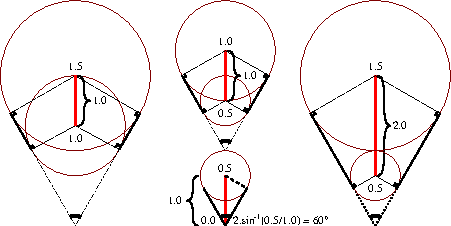
\includegraphics[width=.9\columnwidth]{sources/method/distance_based_angles.pdf}
\caption{MAT explanation by Kao et al.}
\end{figure}

\subsection{Compute MAT}

\begin{figure}
% from /home/t.kuipers/Documents/PhD/Variable_Width_project/pathplanning preliminaries/straight_skeleton_vs_medial_axis.svg
\begin{subfigure}{0.45\columnwidth}
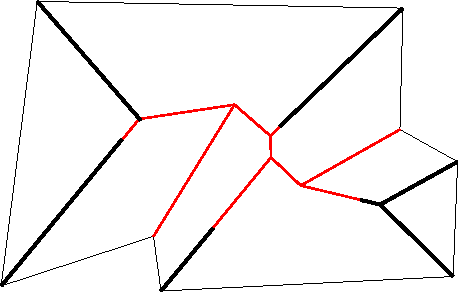
\includegraphics[width=\columnwidth]{sources/method/example_straight_skeleton.pdf}
\caption{Straight skeleton}
\end{subfigure}
\begin{subfigure}{0.45\columnwidth}
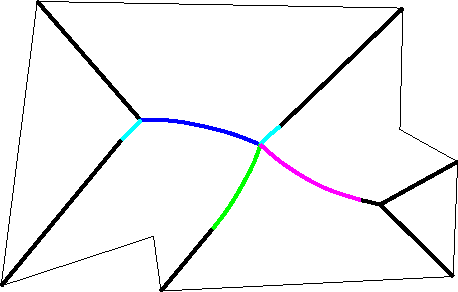
\includegraphics[width=\columnwidth]{sources/method/example_medial_axis.pdf}
\caption{Medial axis}
\end{subfigure}
\caption{Example polygon middle analysis thingies. Difference is colored.}
\label{medial_axis_vs_straight_skeleton}
\end{figure}


\subsubsection{Medial axis rather than Straight Skeleton}
See \cref{medial_axis_vs_straight_skeleton}.
Medial axis handles concave corners differently:
instead of generating the bisector, it will generate a parabolic arc in between the vertex and another line segment of the outline polygon.

\st{Medial axis is stable against small perturbations in the input polygon!}
Concave corners are handled irrespective of how many vertices are in a corner.
\hl{(The medial axis is not stable in that whole new bones can be introduced just by adding a small bump in the outline.)}


$\to$ approximate parabolas for simpler processing!
A straight skeleton can be made to coincide with the medial axis by changing concave corners into an infinitesimal circle arc;
this does introduce a lot of extra bones, though.


The bones of the medial axis which are not directly connected to the outline segment the area in as much sub-areas as the part has polygons.


\begin{figure}
\begin{subfigure}{0.3\columnwidth}
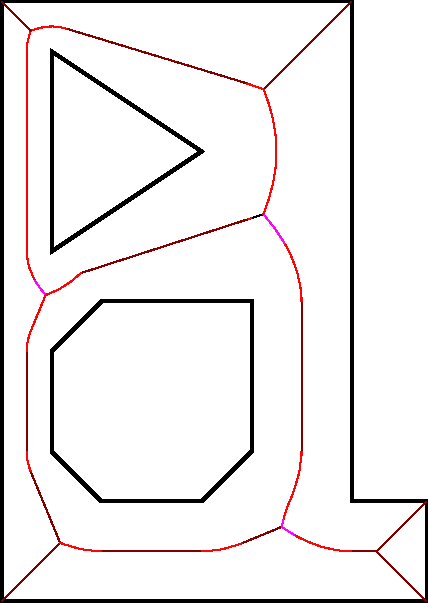
\includegraphics[width=\columnwidth]{sources/method/MAT_example.pdf}
\caption{MAT}
\end{subfigure}
\begin{subfigure}{0.3\columnwidth}
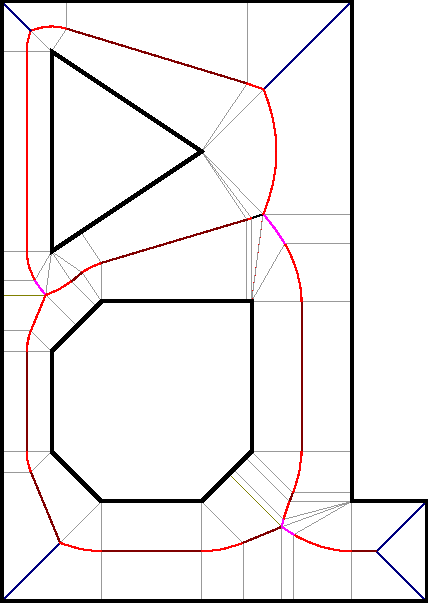
\includegraphics[width=\columnwidth]{sources/method/gMAT_example.pdf}
\caption{gMAT}
\end{subfigure}
\begin{subfigure}{0.3\columnwidth}
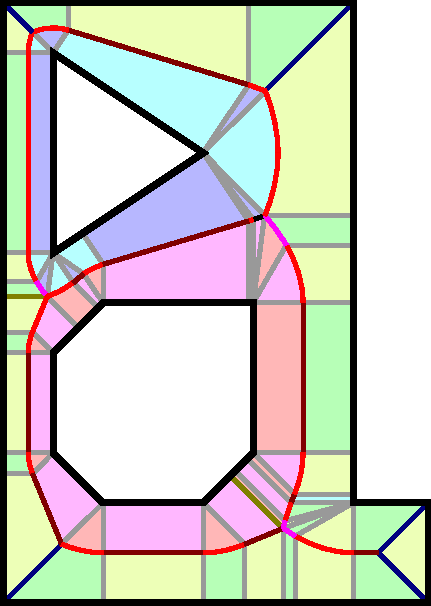
\includegraphics[width=\columnwidth]{sources/method/gMAT_example_labeling.pdf}
\caption{Quads in gMAT}
\end{subfigure}
\caption{Grounded medial axis transform. Dark red are linear segments,  bright red are parabolic segments with high curvature, parabola segments with low curvature are purple. The labelings of areas show that the gMAT divides the area into quads and triangles and that the medial axis divides the area into sub-areas for each outline polygon.}
\label{gmat}
\end{figure}



\subsubsection{grounded Medial Axis Transform}
See \cref{gmat}.
The medial axis is commonly defined either as the set of points with more than one closest point on the boundary or as the set of quench sites of a fire started at the outline polygon growing inward.
A novel way of conceptualizing the medial axis is as a data structure which encodes the distance field.
The medial axis is the set of all points where the derivative of the distance field is discontinuous.

The medial axis transform (MAT) is the combination of the medial axis with at each node the distance values $R$.

We propose a modified MAT: the grounded medial axis transform: gMAT.
The distance field defined by the gMAT approximates the distance field of the MAT using \uwave{piece-wise linear quads}.
The gMAT is the set of all points where the derivative of the distance field is not constant.


Each node in the gMAT is connected to the outline via a \emph{single} bone.
This condition is violated on a MAT where there are concave outline verts.
The gMAT segments the polygon in quads consisting of 1 outline segment and 3 bones, one of which is not directly connected to the outline.
For concave verts the outline segments is missing and the quad becomes a triangle;
likewise for convex sections it may happen that the inner bone is missing from the quad so that it forms a triangle.

For a normal MAT it is already the case that
for a bone segment $v_0 v_1$ generated by two outline segments $p_0 p_1$ and $p_2 p_3$,
the distance on locations along $v_0 v_1$ can be interpolated linearly between $R(v_0)$ and $R(v_1)$.
The distance field between $v_0 v_1$ and $p_0 p_1$ can be constructed linearly as well.

For a MAT the same does not hold for parabolic bones or bones generated by two concave outline verts.
We therefore discretize these segments and connect the introduced nodes to the oulines using new ribs.
The resulting quads encode the original distance field in a piece-wise fashion using linear gradients.


The MAT is a subset of the Voronoi diagram inside the part, which in turn is a subset of the gMAT.
See \cref{voronoi_MAT}.

\begin{figure}
\centering
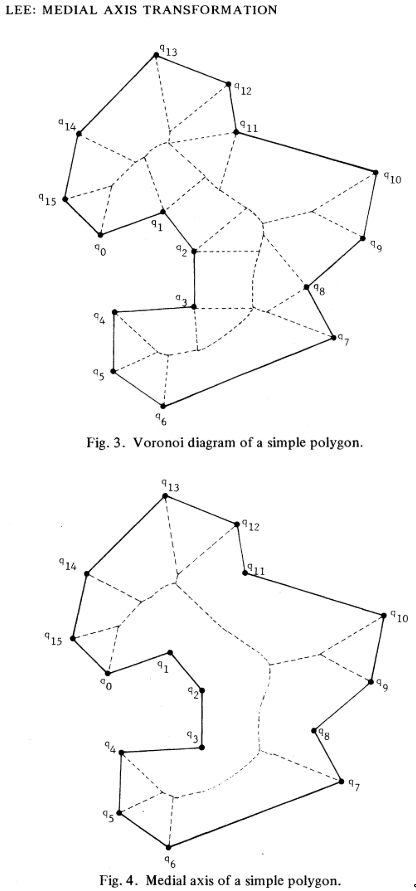
\includegraphics[width=.8\columnwidth]{sources/method/voronoi_MAT.png}
\caption{From \citeauthor{lee1982medial} \cite{lee1982medial}}
\label{voronoi_MAT}
\end{figure}





\subsection{Significance measure}\label{sec:significance_measure}
\Cref{rounded_dist_measures}
We mark bones as to-be-transformed based on the angle between the two edges of the polygon for which this bone is the bisector.
Equivalently we can look at the \emph{bisector angle} $\alpha$ between a skeletal point and the two closest points on the outline.
(Same definition as \cite{attali1996modeling}.)

\paragraph{line-line bones}
When the angle between two outline segments is small, the naive method will produce long triangular gaps.
A computationally efficient way to compute $\alpha$ can be obtained by looking at the ratio between $R$ and Euclidean distance.
Equivalently we can compare the Euclidean distance between two vertices with the difference in distance measure;
if $ |v_1 - v_0| > 2 | R(v_1) - R(v_0) |$ then $\alpha > \SI{120}{\degree}$.

\begin{figure}[H]
\centering
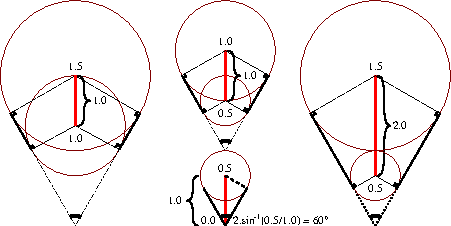
\includegraphics[width=.9\columnwidth]{sources/method/distance_based_angles.pdf}
\caption{Distance based angle estimation. By comparing the euclidean distance between two vertices with the distance measure of the MAT we can skip comparing the angles between the outline segments.}
\label{distance_based_angles}
\end{figure}

The Euclidean distance between two MAT vertices can never be less than the difference in the MAT distance measure between the vertices:t
\begin{figure}[H]
\centering
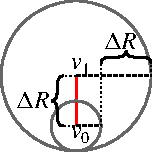
\includegraphics[width=.3\columnwidth]{sources/method/distance_ratio_limit.pdf}
\caption{Minimal Euclidean distance for a given difference in MAT distance measure.}
\label{distance_ratio_limit}
\end{figure}




\paragraph{line-point segments}
For a parabola MAT segment generated by point $(0,d)$ and an outline segment lying on the x-axis, the parabola is given by $y = \frac{1}{2d} x^2 + \frac12 d$.
If $\alpha > \SI{120}{\degree}$ then $\tan^{-1} \abs \partial y / \partial x < \SI{30}{\degree}$,
i.e.  $\tan^{-1} \abs x/d < \SI{30}{\degree}$,
i.e. when $\abs x/d < 1 / \sqrt{3}$,
i.e. when $\abs x < d \sqrt{3} / 3$.
So we mark the part of the parabola as to-be-transformed for which $x \in [-d \sqrt{3} / 3, d \sqrt{3} / 3]$.

\begin{figure}[H]
\centering
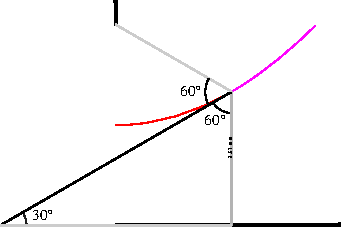
\includegraphics[width=.5\columnwidth]{sources/method/end_of_markings_point_line.pdf}
\caption{End-of-markings for a parabolic spine segment.}
\label{end_of_markings_point_point}
\end{figure}




\paragraph{point-point bones}
For a segment gerenated by points $(0,0)$ and $(0,d)$, the angle $\alpha > \SI{120}{\degree}$ when $\abs(x) < \frac12 d \tan \SI{30}{\degree} $,
so we mark the part of the straight MAT segment as to-be-transformed for which $x \in [-d \sqrt{3}/6, d \sqrt{3}/6]$.

\begin{figure}[H]
\centering
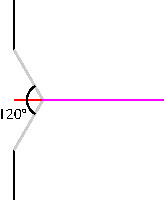
\includegraphics[width=.3\columnwidth]{sources/method/end_of_markings_point_point.pdf}
\caption{End-of-markings for the segment(s) generated by two outline verts.}
\label{end_of_markings_point_point}
\end{figure}







\subsection{Beading strategy}
The next step is to determine how we will fill a given distance between the outline and a significant/marked MAT segment with a whole number of beads. We want to fit an exact whole number of beads in order to prevent a gap being generated.

We need a function $W$ from a given radial distance $R(v)$ to a number of beads and their widths.
These widths depend on the following parameters:
\begin{description}
\item[$\wmin$] the minimum possible bead width
\item[$\wmax$] the maximum possible bead width
\item[$\wout$] the preferred bead width of the outer inset
\item[$\win$] the preferred bead width of the other insets
\end{description}

The function $W$ needs to be able to deal with a range which is considerably shorter than $[\wmin, 2\wmin]$, even so short as to accomodate just $[\win,\win]$ only.
The function needs to be such that we never overshoot the radial distance $R(v)$, because that would affect the dimensional accuracy.
Any distance left over which cannot be filled given the range $[\wmin, \wmax]$ should be placed on the inside near the MAT.

We define $W(d)$ as a sequence of bead widths.
The length of that sequence is $b(d)$.
For example: with $\win = \SI{0.4}{\milli\meter}$ we could have $b(1.05) = 2.5$ and $W(1.05) = (0.4, 0.4, 0.5)$.
The last number is the innermost bead width if there is a singleton bead along the medial axis; only half of that bead spans along a radial distance.

The function $b$ should adhere to several criteria:
\begin{itemize}
\item $b \left( \frac12 n\win \right) = \frac12 n$ for integer $n$
\item $b$ is monotonic
%the item below follows from the two above
% \item between a location with radial distance $R(v) \in [\frac12 n\win, \frac12 (n+1)\win]$ (for integer $n$) there is only one transition to a different number of beads
\item $ 0 \leq b(d) \leq d / w_\text{min} $
\item the width $W(c, d)_n$ of each bead $n$ increases monotonically and gradually in regions with constant bead count $c$: $0 \leq \frac{\partial W(c, d)_n}{\partial d} < \infty$.
\end{itemize}

For our method we also require the inverse $b^{-1}(n)$ which gives the smallest $d$ for which $b(d) = n$.

For our application we define a $W$ adhereing to the following aditional constraints in order of priority:
\begin{itemize}
\item Minimize unfilled area
\item Try to get the outer bead width $W_1$ as close as possible to $\wout$
\item Have the rest of the $W_n$ the same width
\item at transition regions decide between $n$ and $n+1$ beads using the Loss fuction scheme below
\item From a $d$ for which $b(d) = 3$ we don't consider fractional $b(d)$ anymore; we don't allow singleton beads along the medial axis.
\hl{Perhaps we should disallow this because that would require a different transition length}
\end{itemize}

\iffalse
\begin{align}
W(d)_1 = 
  \begin{cases} 
%  \infty & \text{if } w < w_\text{min} \\
   \wout & \text{if } d \geq \wout + \wmin \\
   w - \wmin  & \text{if } 2\wmin  \leq d < \wout + \wmin
  \end{cases}
\end{align}
\fi

%\subsubsection{Optimal beading strategy}
%We could decide on a beading strategy based on some loss function $L$ defined on each line width.

\begin{align}
L(w_1) &= 
  \begin{cases} 
%  \infty & \text{if } w < w_\text{min} \\
   (w - \wout) / (\wmax - \wout) & \text{if } w > \wout\\
   (\wout - w) / (\wout - \wmin)       & \text{otherwise}
  \end{cases}
  \\
L(w_n) &= 
  \begin{cases} 
%  \infty & \text{if } w < w_\text{min} \\
   (w - \win) / (\wmax - \win) & \text{if } w > \win\\
   (\win - w) / (\win - \wmin)       & \text{otherwise}
  \end{cases}
\\
L(W(d)) &= \left(b(d) - \lfloor b(d) \rfloor \right) L \left( W(d)_{\lceil b(d) \rceil} \right)  +  \sum_{n=1}^{n=\lfloor b(d) \rfloor} L( W(d)_n )
\end{align}

(Singular beads are counted only half.)
Together these prioritized constraints uniquely define a single $W$, depending on $\wmin, \wmax, \wout,\win$.
An example is given in \cref{transition_location}.

\begin{figure*}
\centering
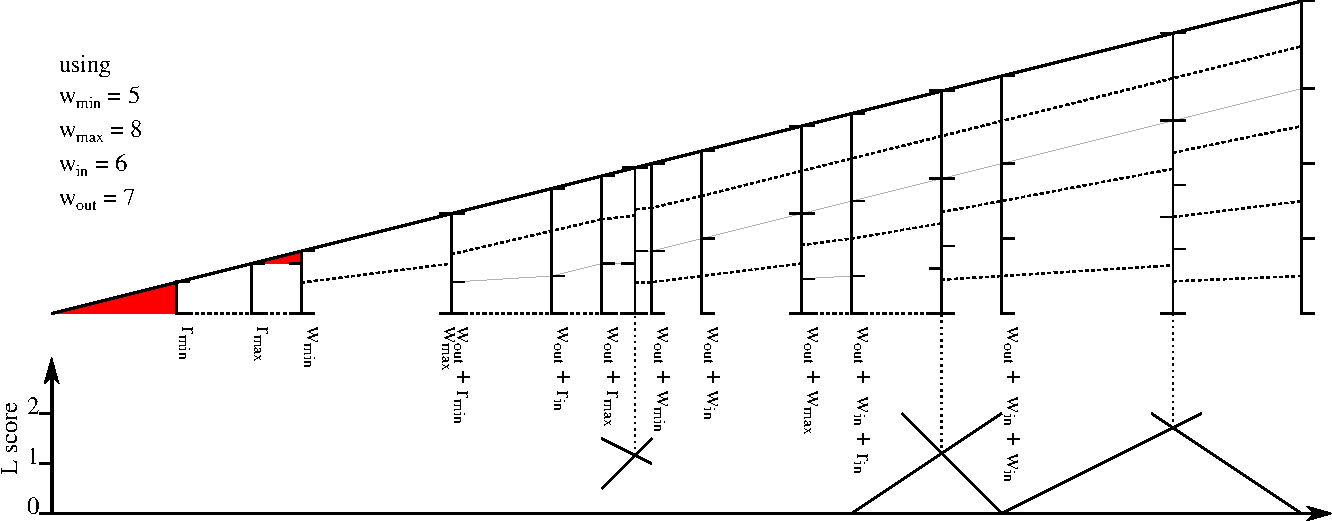
\includegraphics[width=.9\textwidth]{sources/method/ticking_v2.pdf}
\caption{Mapping of different lengths to a ticking. Transition location on a line-line segment is to the right of the middle because the preferred line width is to the left of the middle in the range.}
\label{transition_location}
\end{figure*}

We introduce a function which produces the $d$ at which all widths are prefered: 
\begin{align}
p(n) =
  \begin{cases} 
   \frac12 \wout & \text{if } n = \frac12 \\
    \wout + (n - 1) \win       & \text{otherwise}
  \end{cases}
\end{align}
We call a distance $d$ `prefered' when $d = p(b(d))$


\subsubsection{MAT distance transform}
In order to apply the beading strategy to the MAT
we assign each node $v$ of the medial axis a bead quantity $B^*$ which is initially based on $b(R(v))$, but it is modified in order to prevent discontinuities and remaining gaps.

\hl{How should we define $B^*$? Currently it is always the rounded measure, but it needs to be unrounded in non-marked areas and it needs to support fractional numbers around transitions!}

The bead quantity measure $B^*$ measure should be rounded
where the MAT distance measure $R$ is a local maximum: when all directly connected nodes have a lower MAT distance measure.
See bottom of \cref{rounded_vs_unrounded}.



\subsection{Transitioning}

\begin{figure}
\centering
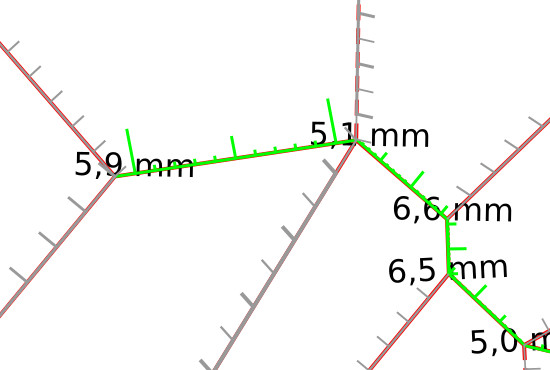
\includegraphics[width=.6\columnwidth]{sources/method/rounded_dist_measures.jpg}
\caption{MAT distance measures at existing joints can be non-integer multiples of bead width.}
\label{rounded_dist_measures}
\end{figure}

See \cref{rounded_dist_measures}.

In order to apply the beading strategy to the MAT, we need a way to smoothly transition to a different number of beads around locations where the 3D model has a changing radius.
The transition will be placed so as to overlap the locations of $b^{-1}(n)$.
We assign each node $v$ of the medial axis a value $b^*$ which is initially based on $b(R(v))$, but it is modified in order to account for transitioning zones.
On the one side of the transition we will have $b^*(v_0)=\frac12 n$ and on the other side we will have $b^*(v_1)=\frac12 n + \frac12$.
For all locations on the MAT in between we linearly interpolate the $b^*$ values, so that we can later interpolate the bead widths $W$ linearly as well.

In a narrow wedge region (a.k.a. a cusp) we have to transfer from $n$ to $n-1$ beads; this transition requires a distance.
See \cref{single_bead_strategy_overview}.
The transition will be such that the innermost toolpath makes a \SI{45}{\degree} angle with the medial axis.
The length of the transition along the medial axis depends on the angles involved.
See \cref{transition_length}.
\begin{equation}
t = r_0 (\sin \alpha + \cos \alpha)
\end{equation}

\begin{figure}[H]
\centering
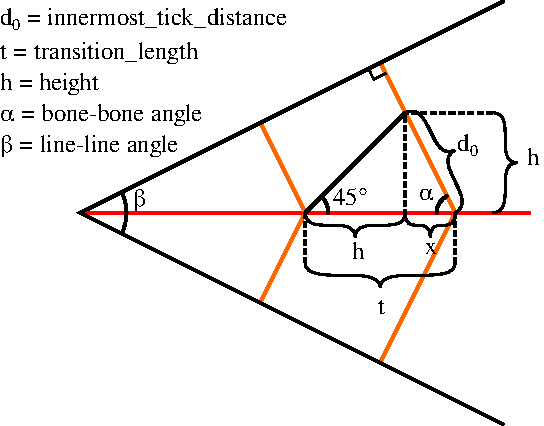
\includegraphics[width=.75\columnwidth]{sources/method/transition_length_v2.pdf}
\caption{Transition length on a line-line segment.}
\label{transition_length}
\end{figure}

The position of the transition is somehwre in between whole tick values.
The relative position in between the whole tick values relates to the relative position of the preferred line width within the range of possible widths.
For a distance $d$ in between a location on the medial axis with a MAT distance of $nr_*$ and one with $(n+1)r_*$ the transition should be positioned around $d - d\frac{r_* - r_-}{r_+ - r_-}$ from the former location.
See \cref{transition_location}.
However, where should the transition be placed precisely? Should the middle of the transition be at that location, or do we again take a relative position of the transition to be at that location?
For extremal values of $r_*$ the transition could overlap with the whole ticks if we simple place the middle of the transition at the specified location.
We therefore place the same ratio of the transition is before the specified location.


\hl{We would like to have a formulation of the MAT distance stransform which defines the MAT distance for any position even if it's not possible to define where the middle of the transition would end up.}
In terms of dMAT/dEuclidean?

The transition needs to be robust against extra fingers in the MAT.
How do we compute the vertex location of an inset on a finger which crosses a transitioning area?
By interpolating the MAT distance between the two ends of the transition, we obtain a stable method for determining the vertex locations of insets.
See \cref{distance_rounding_transition}.
The extra fingers (blue) cause a negligible difference in the inset path (compare the black dashed pat hwith the red dashed path).
\hl{Does this hold for any angled wedge? How about point-line segments or point-point segments?}

\begin{figure}[H]
\centering
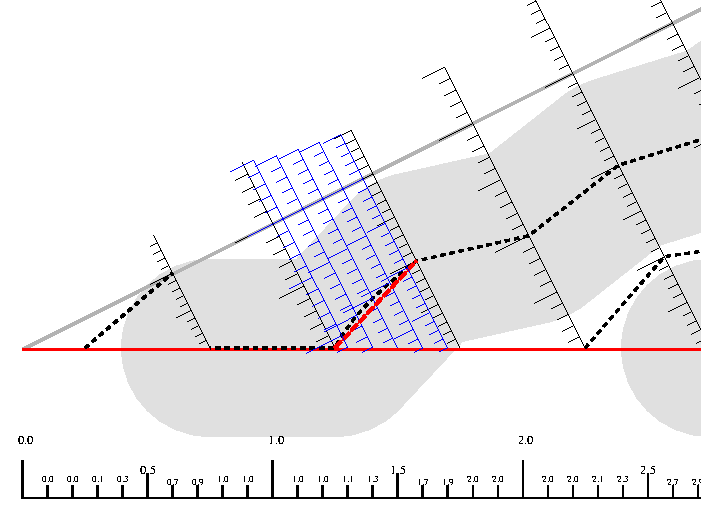
\includegraphics[width=.9\columnwidth]{sources/method/distance_rounding_transition.pdf}
\caption{MAT distance remapping.}
\label{distance_rounding_transition}
\end{figure}


\subsubsection{Ends of markings}
There are multiple ways in which a sequence of bones starting from the outline polygon can be said to end.
\begin{enumerate}
\item The last node in the sequence is a local maximum
\item The last node in the sequence is not connected to a marked segment
\end{enumerate}

The tick quantity measure should be rounded
where the MAT distance measure is a local maximum: when all directly connected nodes have a lower MAT distance measure.
See bottom of \cref{rounded_vs_unrounded}.



For vertices at the end of a sequence of marked MAT segments we need to take care of transitions.
If a transition is overlapping the end of the sequence, then either end of the transition would fall beyond the area where transitions should occur.
How should we deal with thse?
\begin{itemize}
\item We need to keep the transition tick on the marked side, because we need to switch to a different number of ticks somewhere.
Moreover, leaving out the whole transition around end-of-markings would violate the stability principle.
\item The end-of-marking itself will retain its interpolated MAT distance as described above.
\item The transition tick on the non-marked side of discarded.
This means that there will also be no single bead segment leading up to the transition, which coincides with how we deal with non-marked areas.
See \cref{single_bead_strategy}.
\end{itemize}
This method of dealing with end-of-markings can result in gaps slightly larger than usual.
See \cref{change_to_marked}.

\begin{figure}[H]
\begin{subfigure}{0.45\columnwidth}
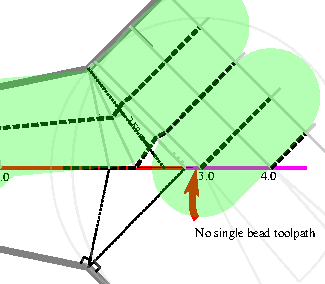
\includegraphics[width=\columnwidth]{sources/method/change_to_marked.pdf}
\caption{before end of markings}
\end{subfigure}
\begin{subfigure}{0.45\columnwidth}
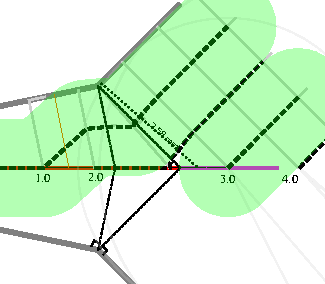
\includegraphics[width=\columnwidth]{sources/method/change_to_marked_2.pdf}
\caption{after end of markings}
\end{subfigure}
\caption{Transition near end of markings. The gap depends on the positioning of the middle of the transition (dotted lines) with respect to the end of the marked areas.}
\label{change_to_marked}
\end{figure}


It impossible for three marked edges to come together.
(Simple case) If 2 edges of the MAT meet then 3 outline segments are involved; lines through those segments form a triangle which cannot have more than two angles less than \SI{60}{\degree}.
However, what if we connect two marked segments using a small non-marked segment?
There is a distance limit based on \cref{distance_ratio_limit}:
the connecting segment is always larger in Euclidean distance than the difference in MAT distance.






\subsection{4. Introduce joints at key MAT dists}
At the locations where the distance measure changes.
We discretize the distance measure field piecewise linear.
In \cref{distance_rounding_transition} we have one piece at MAT dist $0.0$ from bar $0$ to bar $2.5$, than a piece increasing from MAT dist $0.0$ to $1.0$ from bar $2.5$ to $7.5$ etc.

At the end of a marked section we round the MAT distance measure to the nearest integer and introduce a joint there and connect it to the outline using a new finger.
At those places we round the distance measure without applying transitioning, because the end of the transition would lie beyond the marked region.
 
\paragraph{Note}
We could introduce bones implicitly.
Instead of changing the straight skeleton and introducing bones,
we can simply introduce new vertices on the polygon and generate a new straight skeleton.

\textcolor{gray}{
One could think that this means that the method for introducing joints in the original medial axis should be the same method as used for introducing joints on the newly added fingers connected to the joints introduced in the first step!
}
However, the method for introducing joints on the marked regions may differ from the method for introducing joints on the non-marked regions!









\subsection{5. Add ribs for introduced joints}
\textcolor{gray}{
\paragraph{Angle of fingers introduced on the skeleton}
\Cref{finger_angles}
Cannot be optimized.
Always has to be orthogonal to the polygon segment.
Otherwise the algorithm isn't stable w.r.t. extra vertices in the outline.
}
\begin{figure}[H]
\begin{subfigure}{0.45\columnwidth}
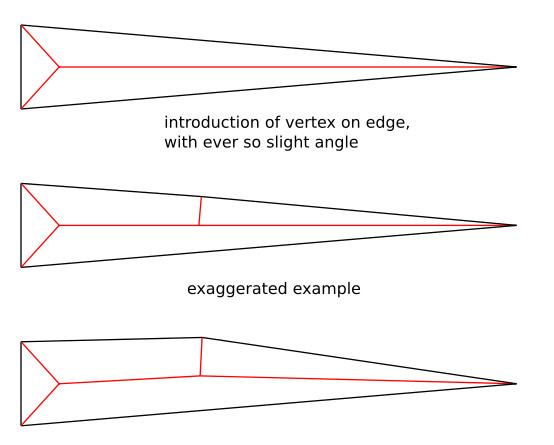
\includegraphics[width=\columnwidth]{sources/method/finger_angles.jpg}
\caption{Stability against extra vertices}
\label{finger_angles_stability}
\end{subfigure}
\begin{subfigure}{0.45\columnwidth}
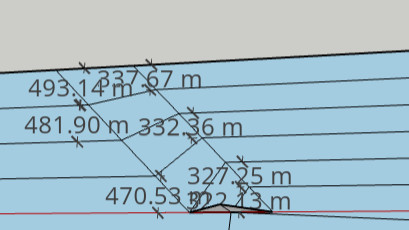
\includegraphics[width=\columnwidth]{sources/method/finger_angles_2.jpg}
\caption{Wrong rib angle, not orthogonal to outline}
\end{subfigure}
\caption{Finger angles should always be orthogonal to the outlines}
\label{finger_angles}
\end{figure}

\begin{wrapfigure}[5]{r}{0.2\linewidth}
\begin{center}
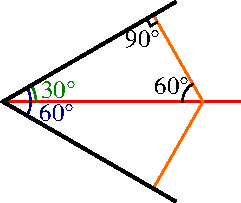
\includegraphics[width=\linewidth]{sources/method/min_angle_of_introduced_bones.pdf}
\end{center}
\end{wrapfigure}

Because the ribs are always orthogonal to the outline segments, the angle $\alpha$ between the spine and ribs is within the range $\SI{60}{\degree} < \alpha < \SI{90}{\degree}$.


\subsection{6. transform MAT distance field}
Before generating the locations we can specify a way to space the integer values non-uniformly along a segment.
We can choose to have bead widths closer to the nominal bead width near lower MAT dists and do the uniform layout only in the upper region of the segment.

This needs to be stable against small perturbations in the outline polygon.
See \cref{heterogeneous_joint_generation}.
For any sequence on non-marked bones from the outline polygon inward we define the stable end point as the first vertex which is connected to a marked medial axis segment.
Based on the MAT distance there we place ticks along the non-marked bones.

\begin{figure}[H]
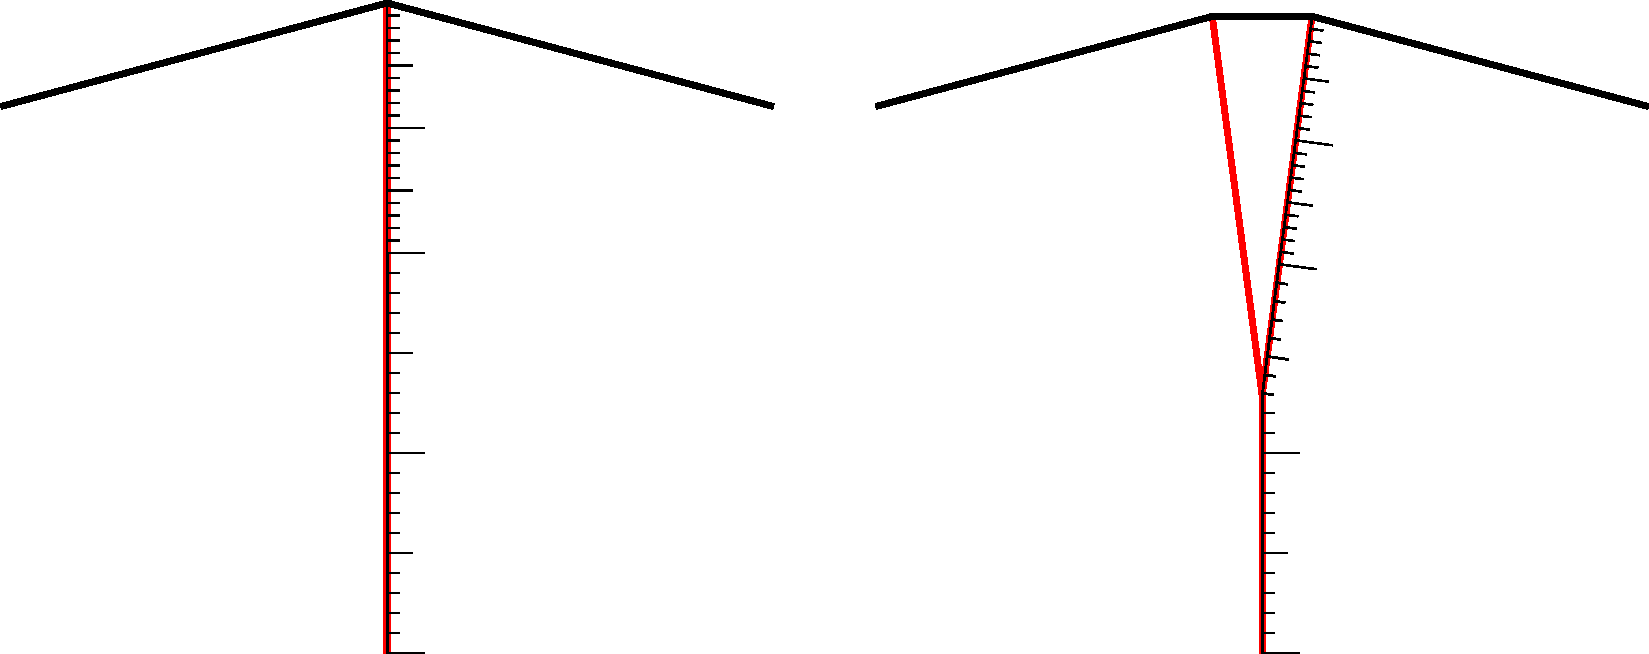
\includegraphics[width=\columnwidth]{sources/method/heterogeneous_joint_generation.pdf}
\caption{Toolpaths employing dist rounding vs without.}
\label{heterogeneous_joint_generation}
\end{figure}






\subsection{7. Location spacing}
\textcolor{gray}{
One could think we should not space the joints evenly along the bones, but make the spacing depend on the angles involved.
We could check the intersection point of the lines of two polygon segments and radially project lines with the same angular spacing.
However, the angular spacing for two patches connected to a single bone would be different, so the paths wouldn't connect!
\hl{Does that mean the angle of the bones should ideally be updated?}
}

\begin{figure}[H]
\centering
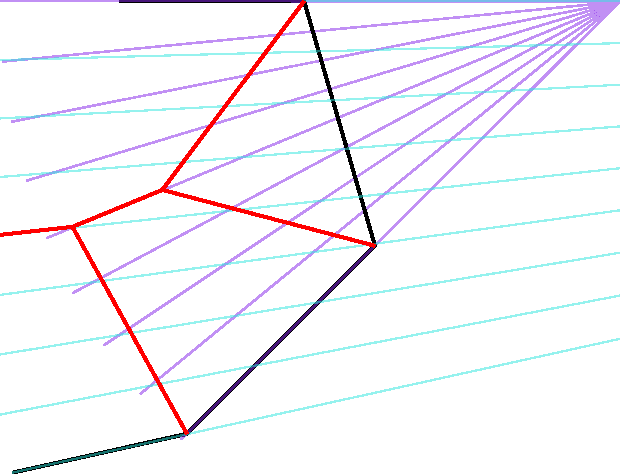
\includegraphics[width=.5\columnwidth]{sources/method/angular_based_spacing.pdf}
\caption{Angular based spacing isn't feasible. The bottom medial axis bone has different spacing based on the two patches. The radially evenly spaced lines are drawn in cyan for the interaction between the bottom outline segment with the top segment and in purple for the interaction between the second bottom segment with  the top segment.}
\label{angular_based_spacing}
\end{figure}


\paragraph{Ideal parabolas}
Subdividing bones introduced for parabolas evenly leads to even spacing along the bone,
while a derived formula seems to produce even spacing in a different sense:
See \cref{medial_axis_parabolas}

\begin{figure}[H]
\begin{subfigure}{0.9\columnwidth}
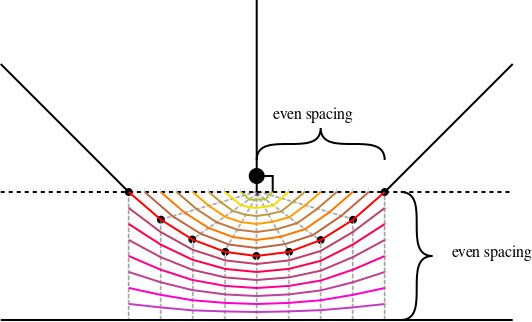
\includegraphics[width=\columnwidth]{sources/method/medial_axis_even_spacing.jpg}
\caption{Parabola transformed to straight skeleton and offsets using even spacing along bones.}
\end{subfigure}
\begin{subfigure}{0.9\columnwidth}
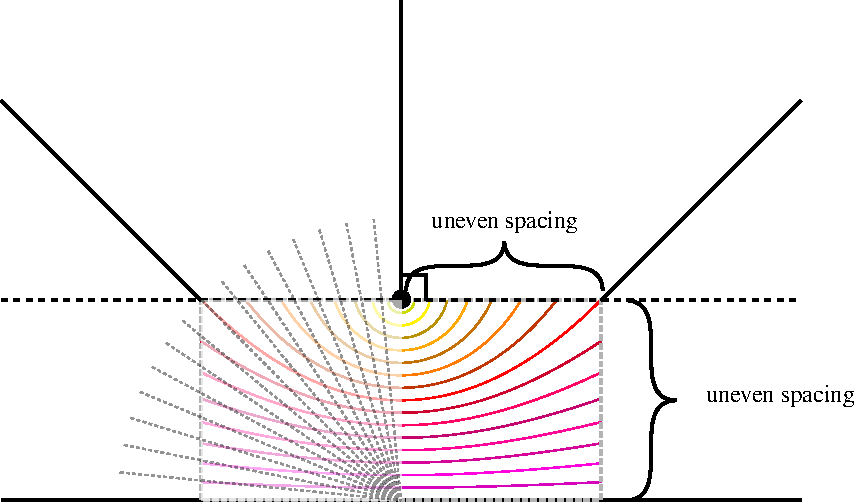
\includegraphics[width=\columnwidth]{sources/method/medial_axis_uneven_spacing.pdf}
\caption{Parabola function plots from analytical solutions where the distance to the point is a whole fraction of the distance to the line.}
\label{medial_axis_parabolas_functions}
\end{subfigure}
\caption{The equidistant points between a vert and a line form a parabola. There are different methods for generating toolpaths which are in between the medial axis and the outline. Note that the uneven spacing does \emph{not} coincide with an even angular spacingat the border between the patches: see the left side of \subref{medial_axis_parabolas_functions}.}
\label{medial_axis_parabolas}
\end{figure}

\hl{But the uneven spacing figure looks like its evenly spaced in the direction orthogonal to the toolpath itself!}






\subsection{8. Connect locations into toolpaths}
\paragraph{Single bead segments}
\Cref{single_bead_strategy}
We round to ingteger multiples of half the nozzle width so as to allow single-bead segments.
These could be printed from polygon and return to polygon over same segment without extruding.
See \cref{single_bead_strategy}.

We only introduce single bead segments along marked areas of the medial axis.
We could also do it for non-marked areas, but that would result in a small single bead segment at \emph{every} corner.


\hl{How to deal with single beads connecting two polys?}
: Print 1st poly $\to$ print single bead $\to$ print 2nd poly $\to$ travel over single bead $\to$ print 1st poly

\hl{How to deal with three-way intersection single beads?}
: Cut up in 1 single bead connecting two polys and 1 normal single bead only connected to one poly


Where to put the middle of the toolpath, based on the middle of the line, the line width and the processing order?


Idea: generate only outer 3 walls, except in marked regions where the distance $R < 5 \win$, so as to prevent jagged infill lines.
Don't generate transitions when $R > 5\win$ or something?
Only do this in skin regions?


\begin{figure}[H]
\centering
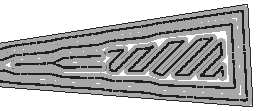
\includegraphics[width=.99\columnwidth]{sources/method/wedge_and_infill.pdf}
\caption{Use single and double wall lines in regions where the infill would be too thin.}
\label{wedge_and_infill}
\end{figure}



\subsection{Overview}
Below in \cref{parabola_switch_to_less_lines} you can see the different technique preliminaries thought out.
The problem this paper is trying to solve is the large gap in M0.
M1, M2 and M3 use vertices at specific locations and use altered distance measures for those points; these methods are not stable to adding more bones to the skeleton.
M4 and M5 define distance measures in any location (based on \cref{distance_rounding_transition}) which makes them stable.
M5 avoids jagged lines by only applying the MAT distance remapping up to a cutoff point discussed in \cref{sec:significance_measure}.


\begin{figure*}
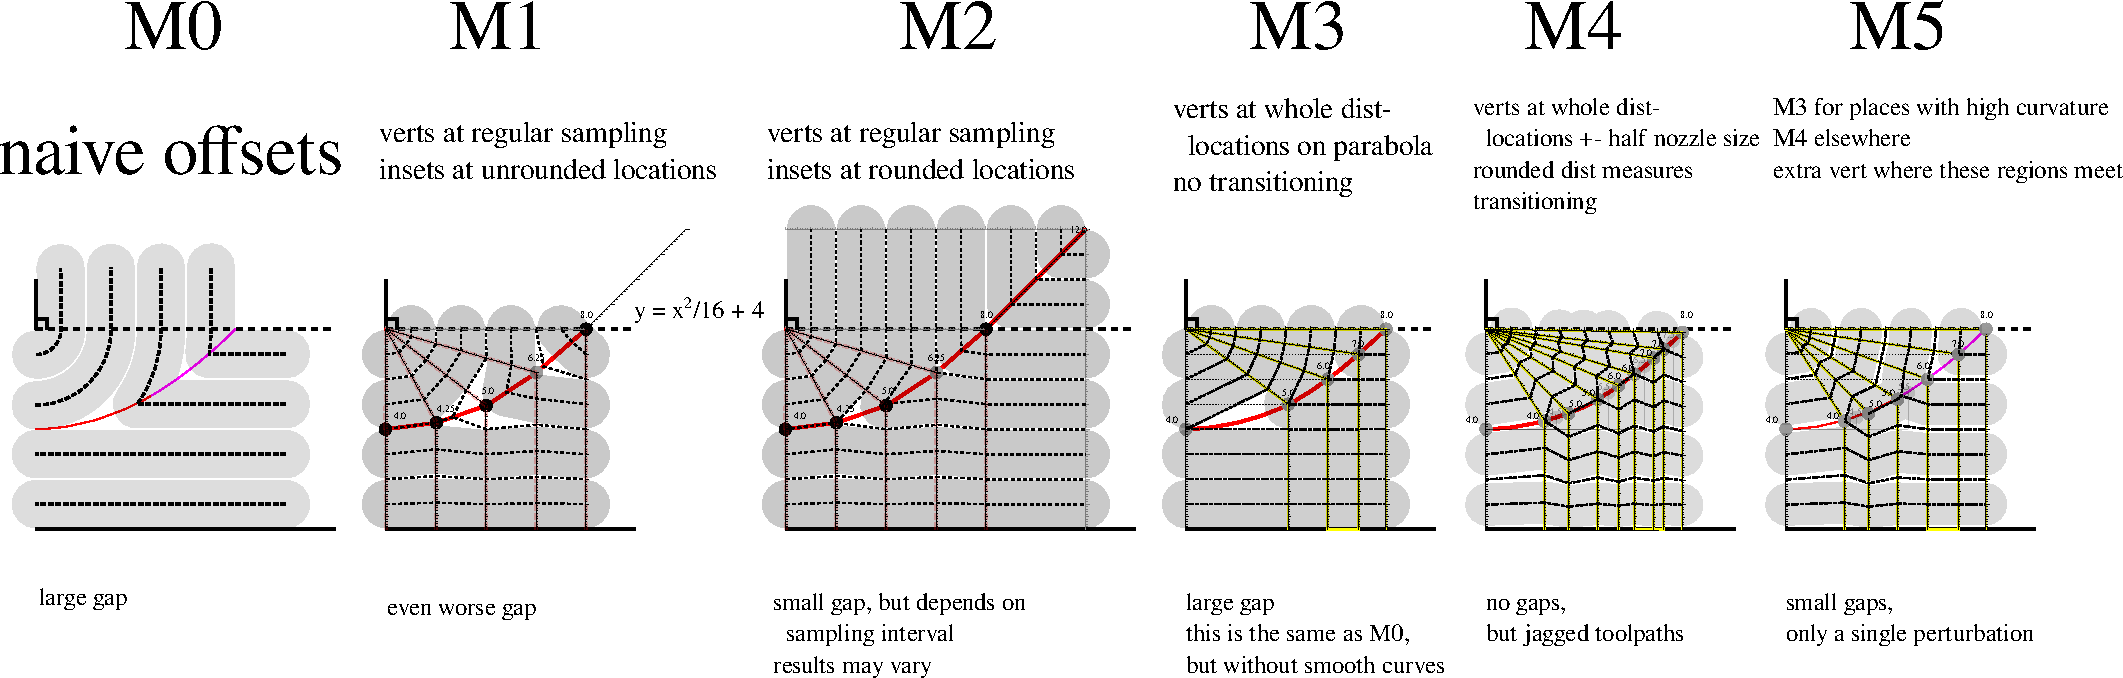
\includegraphics[width=\textwidth]{sources/method/parabola_switch_to_less_lines.pdf}
\caption{Different preliminary variants of the proposed algorithm on a parabola segment.}
\label{parabola_switch_to_less_lines}
\end{figure*}

























































